\documentclass[a4paper,10pt]{article}
\usepackage{graphicx}
\usepackage{amsmath}
\usepackage{subcaption}
\usepackage{hyperref}

\title{EDW Assignment - 1: 7-Segment Display Logic Mapper}
\author{MAHIB - 2023UEC2569}
\date{January 2025}

\begin{document}

\maketitle

\section*{Objective}
The objective of this assignment was to design a schematic involving a 4-input DIP switch, a custom logic mapper, and a 7-segment display. The project required creating Boolean expressions for the custom logic mapper and connecting the outputs to the respective inputs of a 7-segment display.

\section*{Schematic Overview}
The schematic consists of four input signals labeled \(A\), \(B\), \(C\), and \(D\). These inputs are connected to a 4-input DIP switch, which allows the user to toggle between different logic states. The outputs from the DIP switch are then fed into a custom logic mapper, which calculates the values for seven output signals: \(a\), \(b\), \(c\), \(d\), \(e\), \(f\), and \(g\). These outputs are connected to the respective inputs of the 7-segment display.

To access the schematic and the symbol itself, please check out my \href{https://www.github.com/mahib1/EDW_Semester4}{Github Repository}!

\subsection*{Logic Mapper}
The logic mapper consists of the following Boolean equations for the seven outputs:

\[
a = B'D' + BC + AD' + A'C + AB'C' + A'BD
\]
\[
b = B'D' + B'C' + A'CD + AC'D + A'C'D'
\]
\[
c = AB' + C'D + A'B + A'D + B'C'
\]
\[
d = BCD' + ABC' + B'C'D' + BC'D + A'B'C' + B'CD
\]
\[
e = B'D' + CD' + AB + AC
\]
\[
f = AB' + BD' + AC + C'D' + A'BC'
\]
\[
g = CD' + AB' + B'C + AD + A'BC'
\]

\section*{7-Segment Display}
The outputs from the logic mapper are connected to the respective red inputs of a 7-segment display. The common anode input of the display is connected to \(V_{cc}\) (5V), with a 220-ohm resistor in series to maintain the required 2V potential difference across the LEDs in the display.

\section*{Schematic and Custom Symbols}

Below are the images for the schematic design and the custom symbols used in the project. Each image is displayed as a subfigure.

\begin{figure}[h!]
    \centering
    \begin{subfigure}[b]{0.45\textwidth}
        \centering
        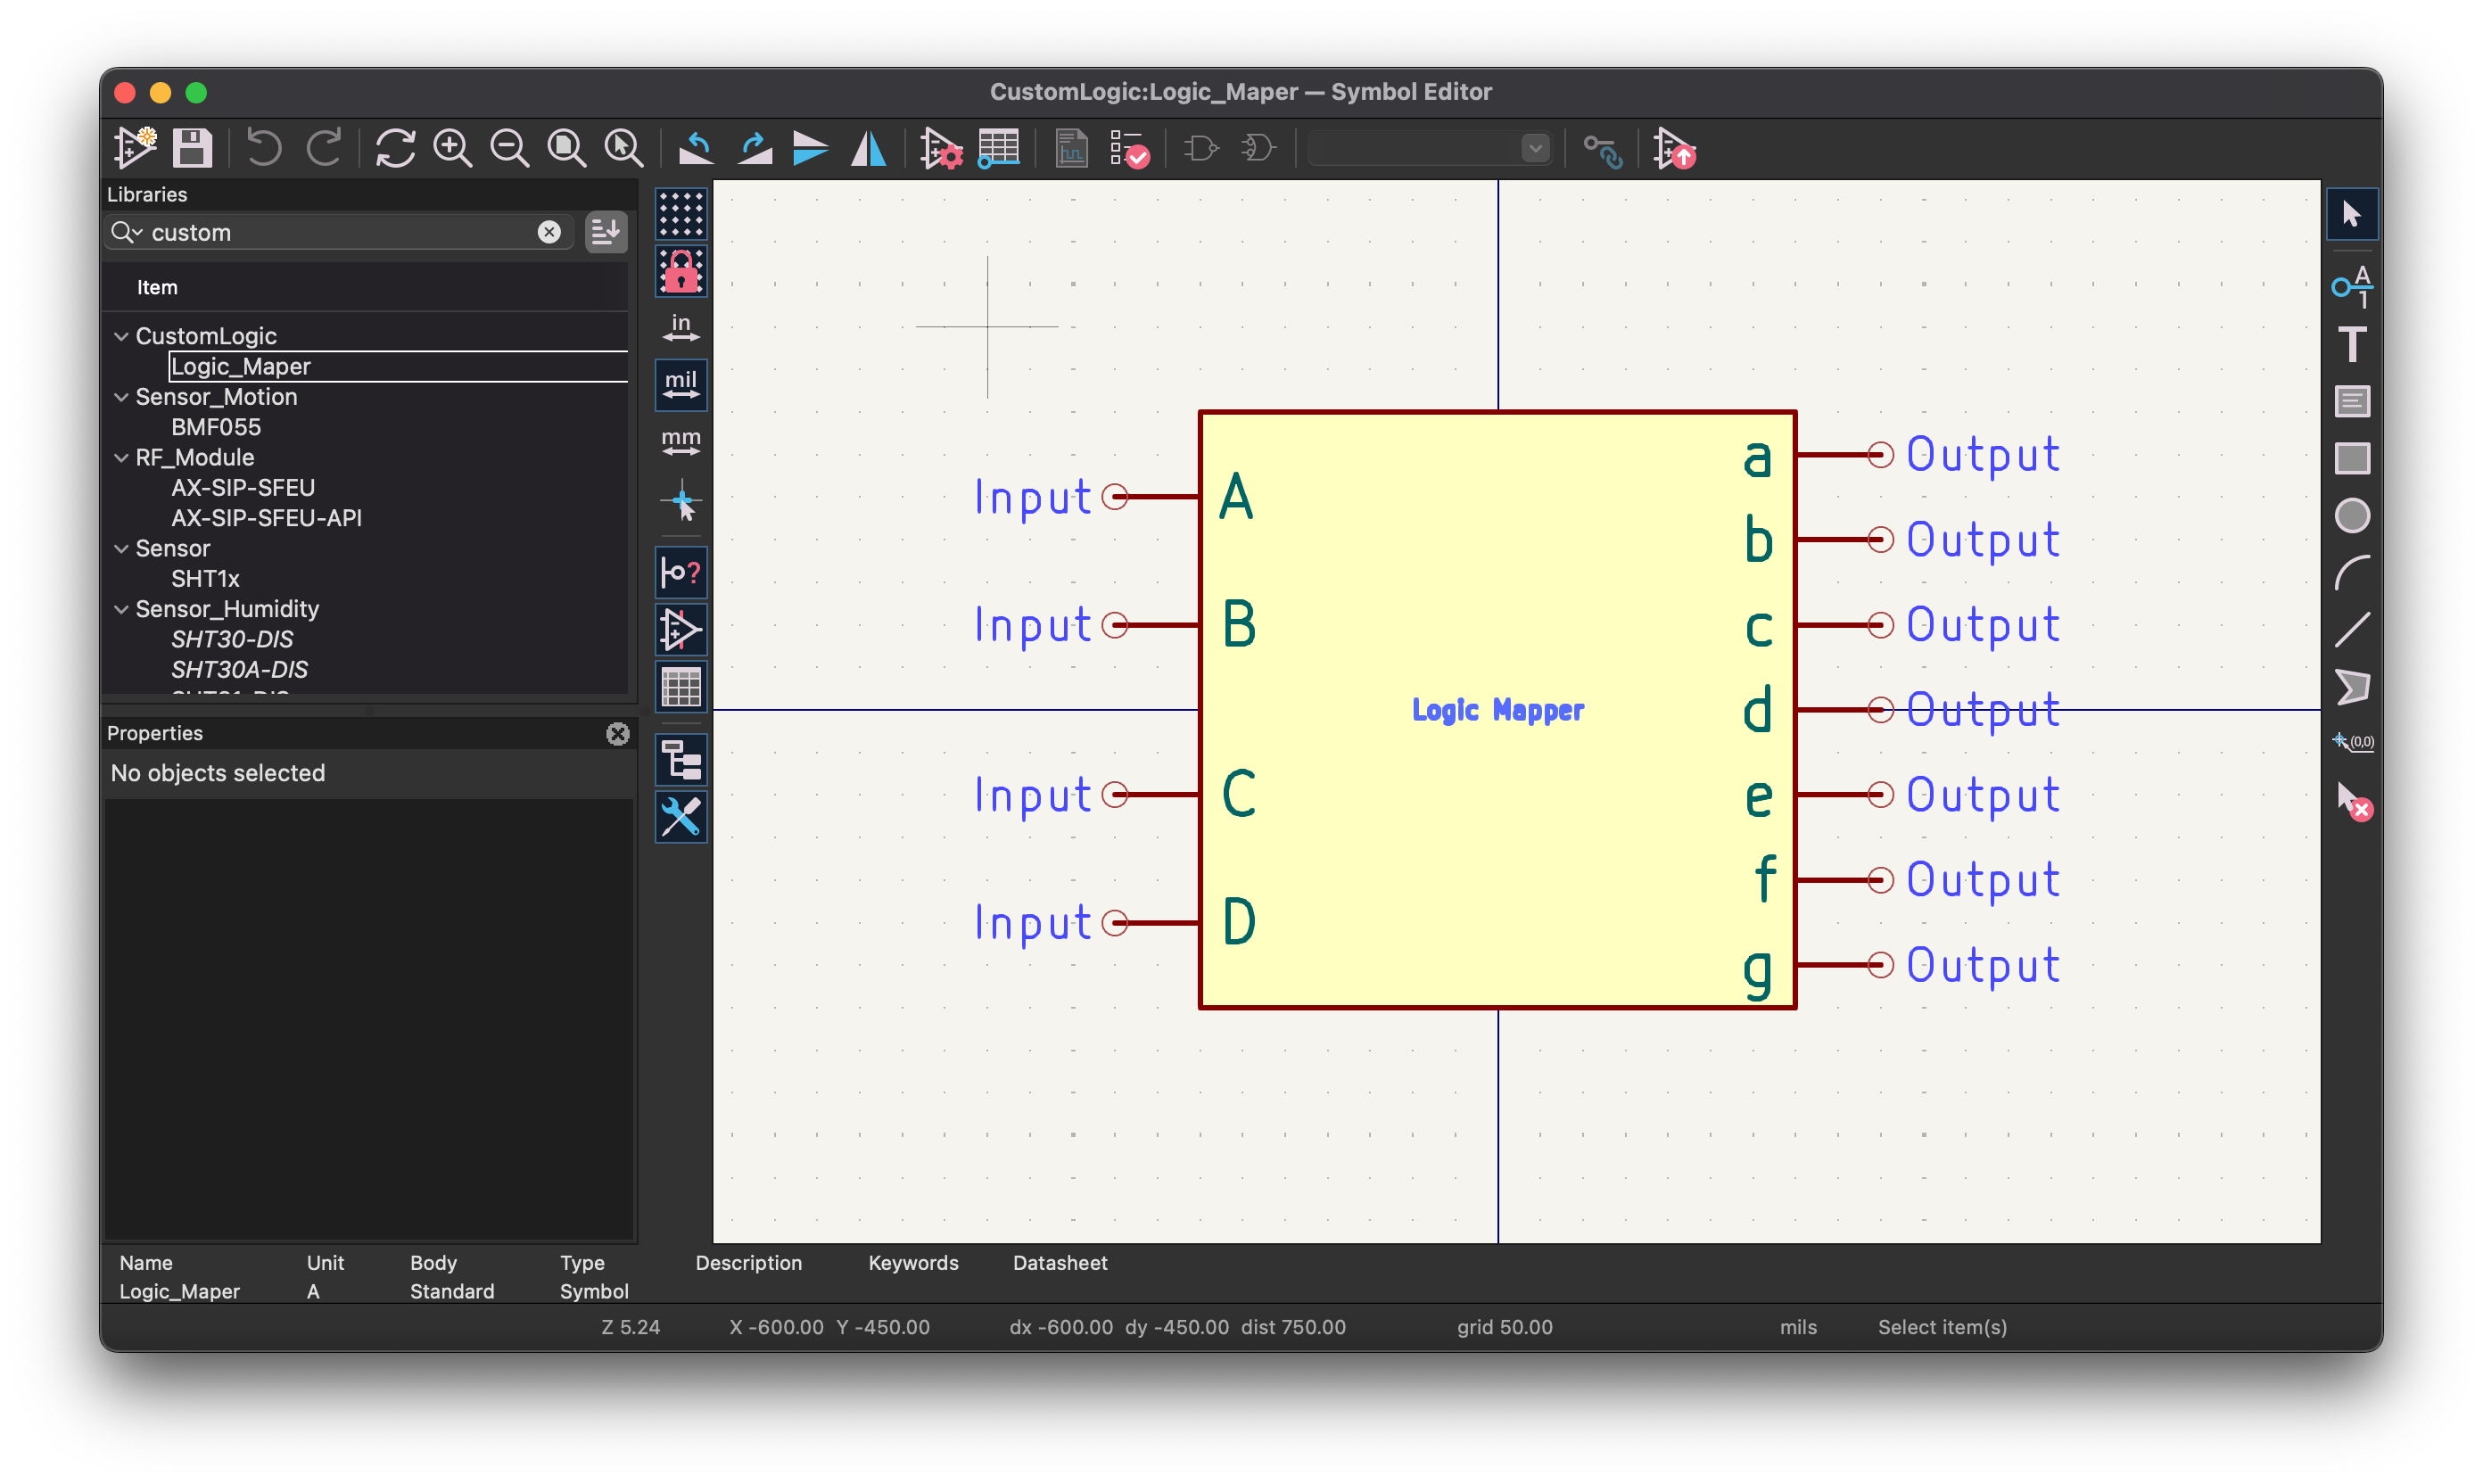
\includegraphics[width=\textwidth]{img/CustomSymbol.png}
        \caption{Logic Mapper Custom Symbol}
        \label{fig:schematic1}
    \end{subfigure}
    \hfill
    \begin{subfigure}[b]{0.45\textwidth}
        \centering
        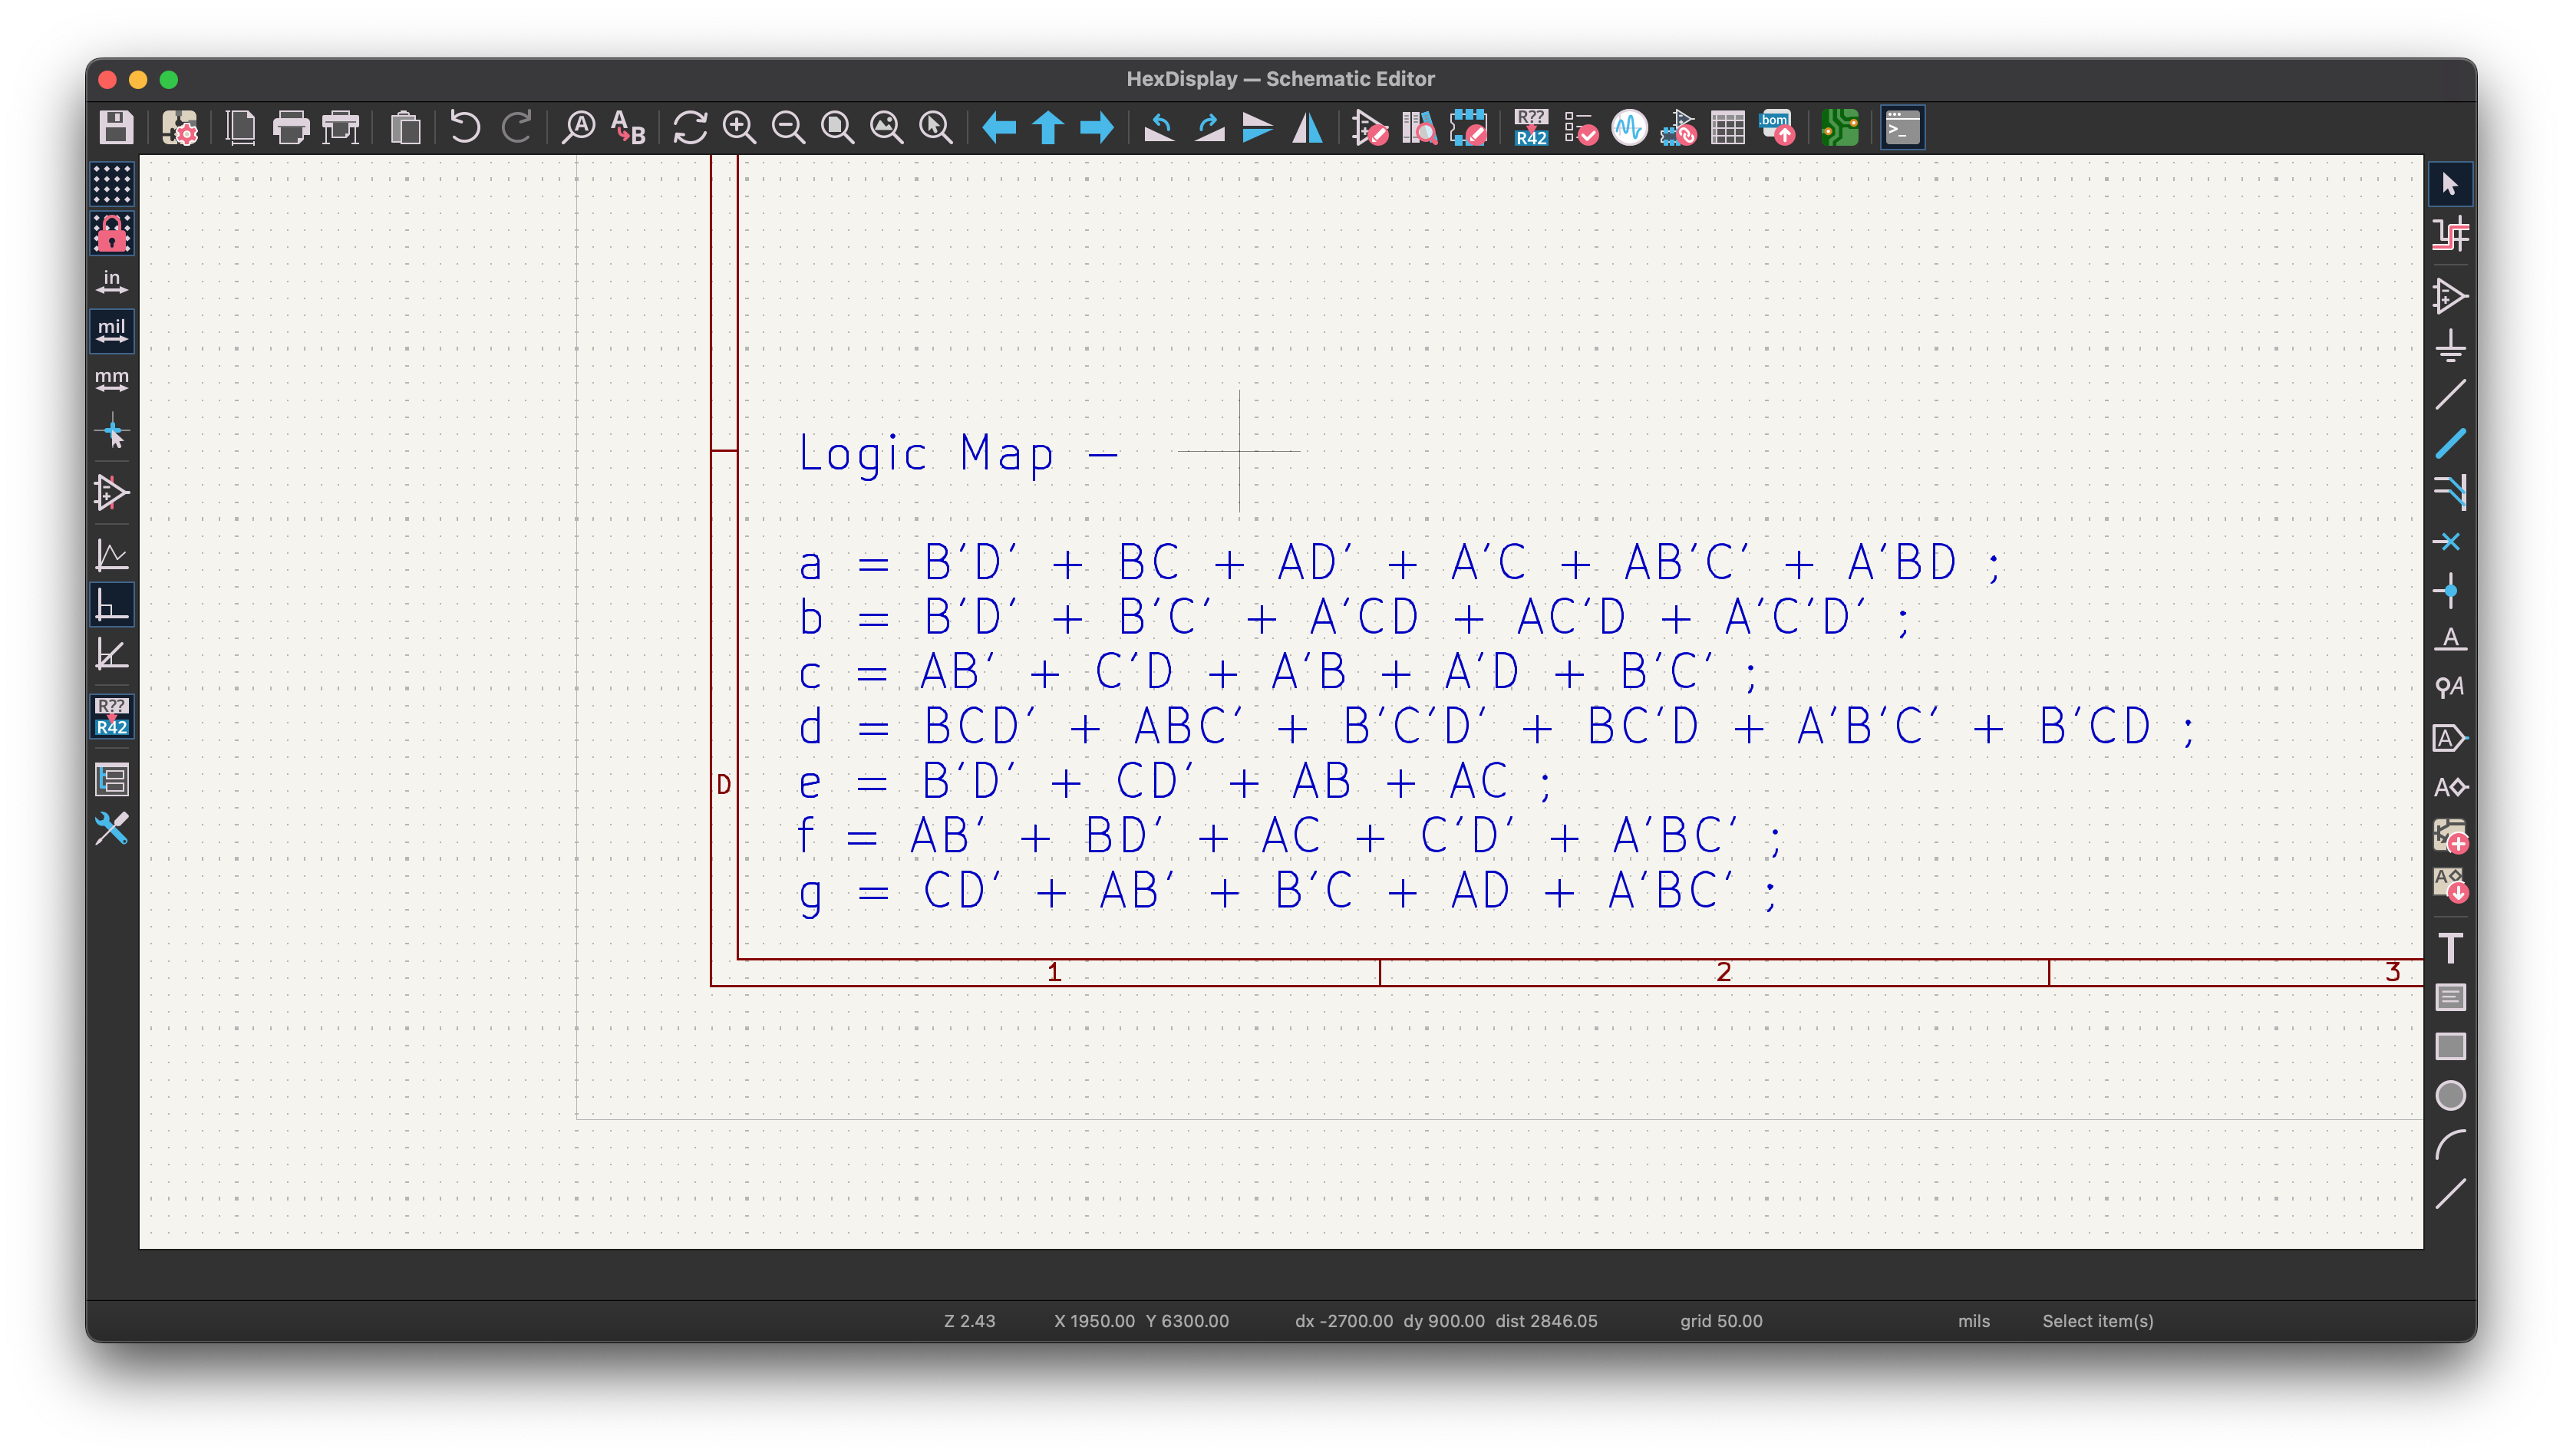
\includegraphics[width=\textwidth]{img/LogicMap.png}
        \caption{Logic Mapper Equations}
        \label{fig:schematic2}
    \end{subfigure}
    
    \vskip\baselineskip
    
    \begin{subfigure}[b]{0.45\textwidth}
        \centering
        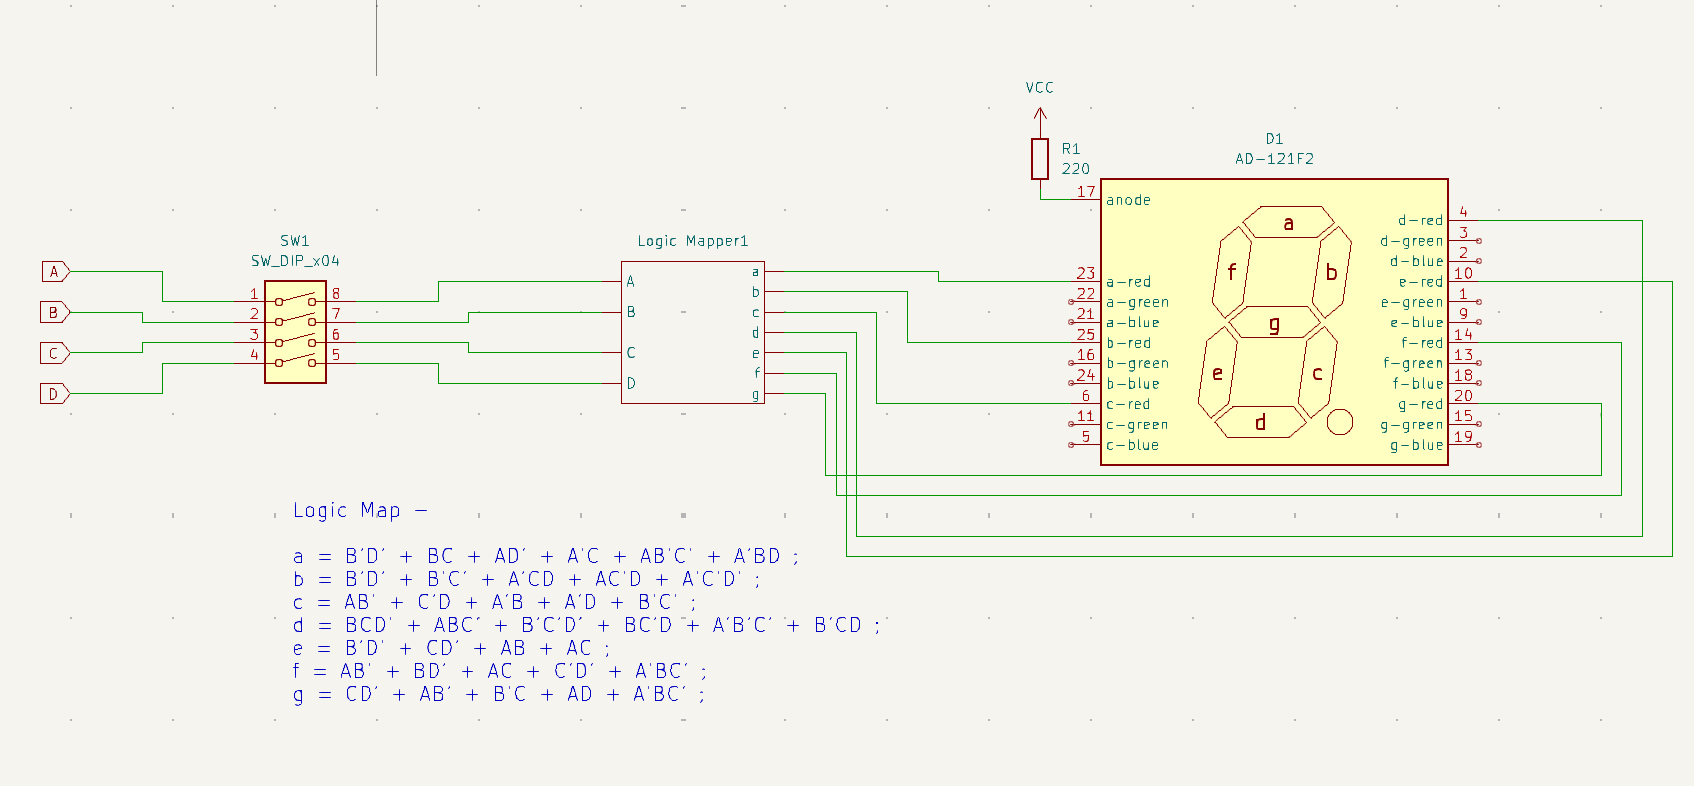
\includegraphics[width=\textwidth]{img/schDiagram.png}
        \caption{Schematic}
        \label{fig:custom_symbol1}
    \end{subfigure}
    \hfill
    \begin{subfigure}[b]{0.45\textwidth}
        \centering
        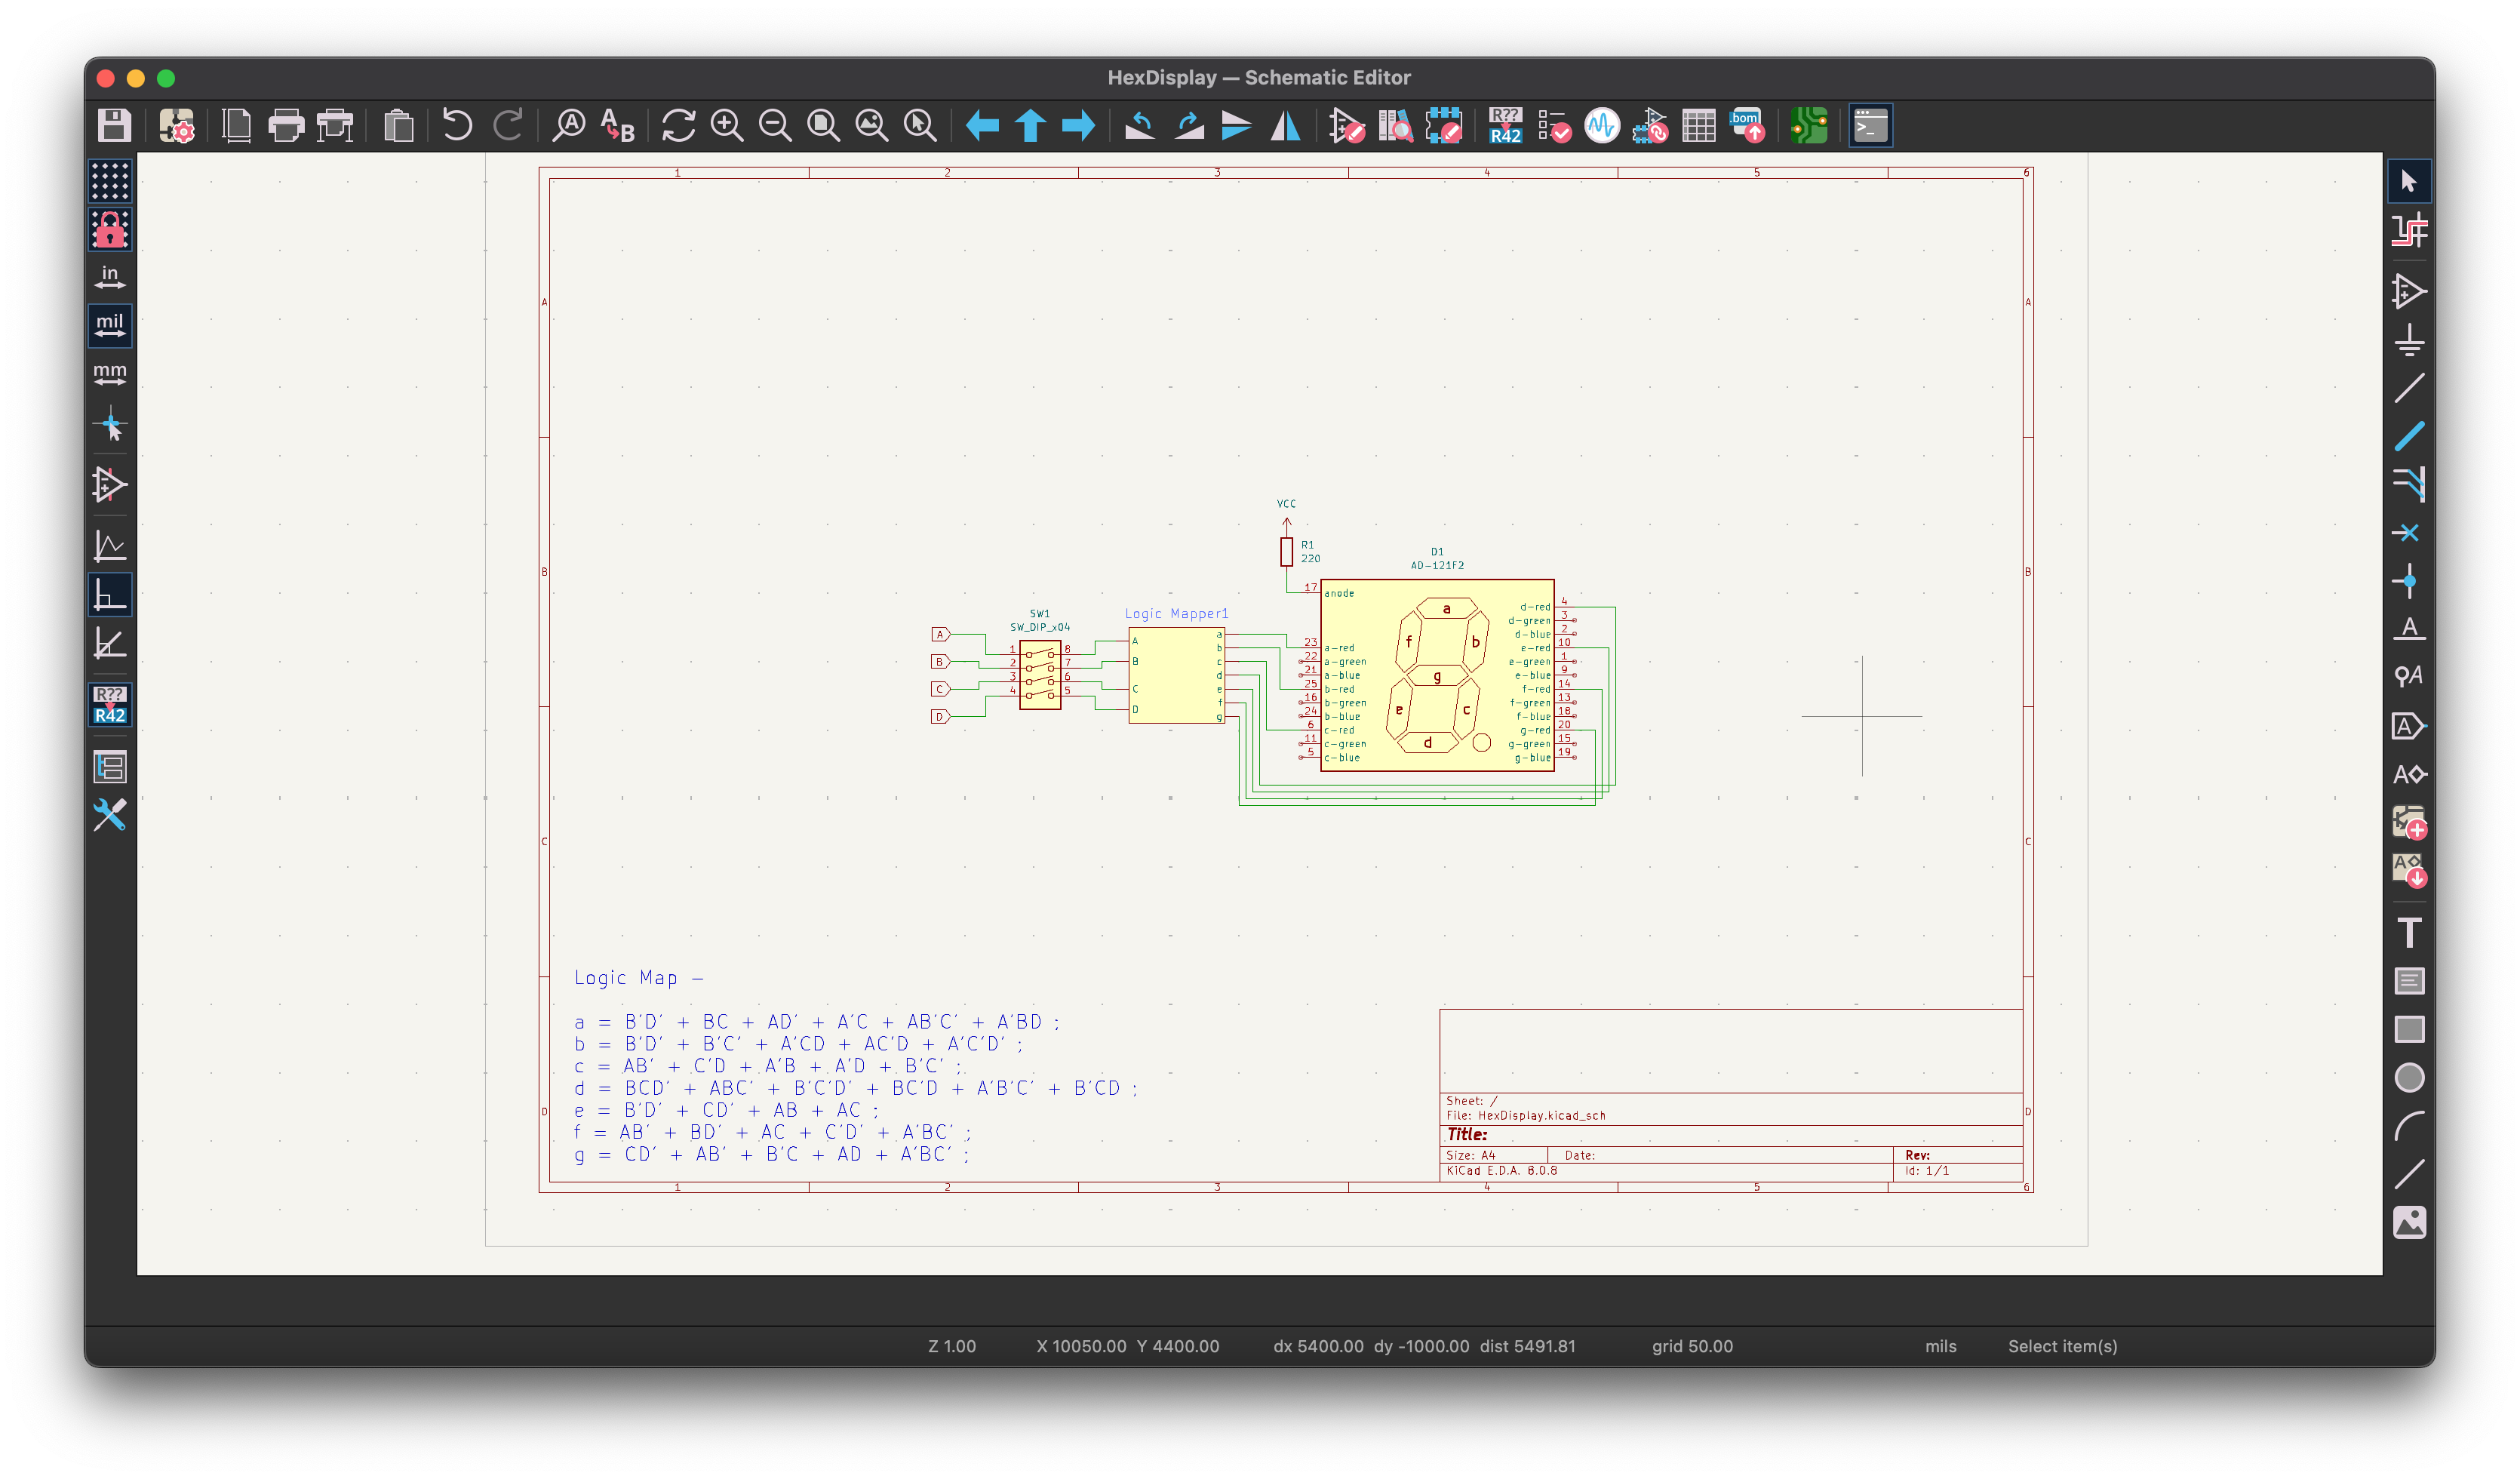
\includegraphics[width=\textwidth]{img/FullSch.png}
        \caption{Full Schematic}
        \label{fig:custom_symbol2}
    \end{subfigure}
    
    \caption{Schematic and Custom Symbols}
    \label{fig:all_images}
\end{figure}

\section*{Conclusion}
This assignment allowed me to design a complex logic circuit with multiple inputs and outputs, and connect them to a 7-segment display to visualize the results. The custom logic mapper was designed using Boolean expressions and the 7-segment display was wired with the appropriate components to display the output in a readable format.\\

A link to all my assignments will be linked right \href{https://www.github.com/mahib1/EDW_Semester4}{here in this repository}!

\end{document}
